
\chapter{Scrolls and the curves they contain}
\label{ScrollsChapter}

If you've never read T. S. Eliot's {\it Old Possum's Book of Practical Cats}, 
you could do worse than start with ``The naming of cats'',
where the poet tells us that
\begin{quote}%
The Naming of Cats is a difficult matter [\dots]\\
a cat must have THREE DIFFERENT NAMES
\end{quote}%

\noindent %leave blank line above so the skips above and below quote match
\emdash one for daily use, one complex and unique, and one ineffable.
So it is with the class of varieties
\index{Eliot @Eliot, Thomas Stearns}%
\index{rational!normal scroll}%
\index{scroll}%
known as \emph{rational normal scrolls}. Although they're some of the
\index{scroll|(}%
simplest subvarieties in projective space\emdash the first examples
are shown in Figure~\ref{Fig16.1}\emdash they have a deeper aspect and
myriad applications (for instance, in describing the embeddings of
curves of low degree and genus), and can be examined from three rather
different points of view, each useful in a different context. We
%
\begin{figure}[h]
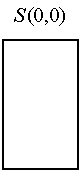
\includegraphics[height=0.8in,trim=0 0 0 15,clip]{main/Fig16-1A}\qquad
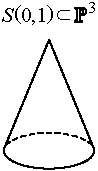
\includegraphics[height=0.8in,trim=0 0 0 15,clip]{main/Fig16-1B}\qquad
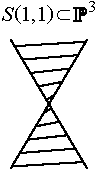
\includegraphics[height=0.8in,trim=0 0 0 15,clip]{main/Fig16-1C}\qquad
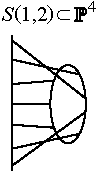
\includegraphics[height=0.8in,trim=0 0 0 15,clip]{main/Fig16-1D-new}%
\caption{The smallest scrolls: from the left, $S(0,1) \cong \PP^{2}$;
$S(0,2)$, the cone over a conic; $S(1,1)\subset \PP^{3}$, the union of
lines joining corresponding points of two skew lines, isomorphic to a
\index{skew lines!in $\symbb P^3$}%
smooth quadric; and $S(1,2)\subset \PP^{4}$, the union of the lines
joining corresponding points on a line and a conic.
\vspace*{-10pt}
}
\label{Fig16.1}
\end{figure}
%
will take up each in turn.%
\footnote{However, we claim no secret knowledge comparable to the
feline name ``that no human research can discover-- But THE CAT
HIMSELF KNOWS.'' The full text of Eliot's poem is available at
https://poets.org/\allowbreak poem/naming-cats.%
}%

{\it In this chapter 
we will refer to rational normal scrolls simply as scrolls.}
We first give
a classical geometric construction, then an algebraic description that
allows one to ``find'' the scrolls containing a given variety, and
then a more modern geometric definition that makes it easy to
understand the divisors on a scroll. Finally, we turn to some of the
applications to the embeddings of curves. We will focus on the case of
2-dimensional scrolls because this is the 
one
that occurs most often in our applications.

\section{Some classical geometry}\label{daily name}

To construct a scroll of dimension 2 in $\PP^r` `$, we start by choosing
integers 
$a_1\ge\nobreak0$
and  
$a_2\ge1$
with $a_1 + a_2 = r-1$, and
consider  a pair of complementary linear subspaces $\PP^{a_1}$ and
$\PP^{a_2} \subset \PP^r = \PP(V)$\emdash that is, we express an
$(r+1)$-dimensional vector space $V$ as a direct sum $V =  V_1 \oplus
V_2$ of subspaces $V_1, V_2 \subset V$ of dimensions $a_1+1$ and
$a_2+1$. For simplicity we will always assume, without loss of 
generality, that $a_{1}\leq a_{2}$.

Next, for $i`=`1,2$, we take $\phi_i \!:\!  % avoid very underfull line
\PP^1 `\to` \PP^{a_i}$ to be the
parametrization of the rational normal curve of degree $a_i$ given by
a basis of homogeneous polynom\-ials of degree $a_i$ (if $a_i = 0$ this
is just the constant map from $\PP^1$ to a point). Finally, we define
the scroll $S(a_1, a_2)$ to be the union of the lines
$$
S(a_1,a_2)\colonequals\bigcup_{p\in \PP^1} \overline{\phi_1(p)\, \phi_2(p)}.
\vspace*{-2pt}
$$
We call the curve $C_{a_{1}}$ a \emph{directrix} of the scroll; if $a_{1}<a_{2}$ this
is unique. 
\index{directrix}%
The family of lines
$ \overline{\phi_1(p) \phi_2(p)}$ is called a 
\index{ruling}%
\emph{ruling} of the scroll, and this is unique except when $a_{2} = 1$,
the case of $S(0,1) = \PP^{2}$, 
and the case of a smooth quadric surface in $ S(1,1)\subset \PP^{3}$.

In the degenerate case $a_{1}= 0$, the surface $S(0,a_{2})$ is the cone
in $\PP^{a_{2}+1}$ over a rational normal curve of degree $a_{2}$.
 Since $S(0,a_2)$ is singular when $a_2\geq 2$,
it is useful to consider the surface
$$
\tilde S(0, a_2) \colonequals  \bigl\{@ (t, q) \in \PP^1 \times \PP^r
\mid q \in \overline{\phi_1(t), \phi_2(t)}@\bigr\}.
$$
This is the 
\index{blowup!of a cone}%
blowup of the cone $S(0, a_2)$ at its vertex; like the
surfaces $S(a_1,a_2)$ with $a_1 > 0$ it is a $\PP^1$ bundle over $\PP^1$
and thus is smooth. As we shall see, $\tilde S(0, a_2)$ is isomorphic
to the scroll $S(1, a_2+1)$.
It is not hard to prove directly that $S(a_1,a_2)$ is an algebraic
variety, and we shall soon write down its defining equations.

From the description above we can immediately deduce the dimension and
degree of a scroll:

\begin{proposition}
\begin{enumerate}
\item $S(a_1,a_2)$ is a nondegenerate surface.
\item $S(a_1,a_2)$ has degree $a_1+a_2$, and codimension $a_1+a_2-1$.
\item $S(a_{1},a_{2})$ is nonsingular if $a_{1}>0$.
\unif
\end{enumerate}
\end{proposition}

\begin{proof}
The rational normal curves separately span the spaces $\PP^{a_i}$, so a
hyperplane containing both of them would contain $\overline{\PP^{a_1},
\PP^{a_{2}}} = \PP^r` `$, proving nondegeneracy.

It is clear from our description that $S$ is 2-dimensional, and thus of
codimension $a_{1}+a_{2}+1 -2 = a_{1}+a_{2}-1$.

To compute the degree, we choose a general hyperplane $H$ containing
$\PP^{a_{1}}$. The intersection $H\cap C_{2}$ consists of $a_{2}$
reduced points. Thus the intersection $H\cap S$ consists of $C_{1}$
and the $a_{2}$ reduced lines connecting
the points of $H\cap C_{2}$ with their corresponding points on $C_{1}$;
this union has degree $a_{1}+a_{2}$.

If $0< a_{1}$ we also see from this argument that, given any point  $p\in
S(a_{1},a_{2})$, there is
a hyperplane section that is nonsingular at $p$, and thus $S(a_{1},a_{2})$
is nonsingular at $p$.
\end{proof}

A completely parallel construction creates 
scrolls of
any dimension $s$. Start with a series of integers $0 \leq a_1 \leq
\dots \leq a_s$;
\label{thescroll}
set $r + 1 = \sum_{i=1}^{s}(a_{i}+1)$,  and
decompose $\CC^{r+1}$ as
$$
\CC^{r+1} = \bigoplus_{i=1}^{s}\CC^{a_{i}+1}.
$$
Let $\PP^{a_{i}}\subset \PP^{r}$ be the subspaces corresponding to the
summands,  choose for each~$i$ a
map $\phi_i : \PP^1 \to \PP^{a_{i}}$  given by a basis of homogeneous
polynomials of degree $a_i$, and define the scroll $S \subset \PP^{r}$ by
$$
S=S(a_{1}, \dots, a_{s}) \colonequals  \bigcup_{p\in
\PP^{1}}\overline{\phi_1(p), \phi_{2}(p), \dots, \phi_{s}(p)}.
$$
For example, $S(a_{1})$ is the rational normal curve of degree $a_{1}$. In
general, the variety $S$ is nondegenerate of codimension $r-s$ and degree
$\sum a_{i} = r-s+1$. The proof is similar to the one we gave for $s=2$.

To put this construction in context, we recall that by
Corollary~\ref{minimal degree bound}
Any irreducible, nondegenerate variety $X$ of codimension $c$ in
$\PP^{r}$ has degree $\geq c +1$.

Thus scrolls are \emph{varieties of minimal degree}. The reader already
\index{minimal degree}%
\index{variety, convention on!of minimal degree, classification}% hack
knows that the rational normal curves of degree $a$ in $\PP^{a}$ are the
only irreducible, nondegenerate curves of degree $a$ and codimension
$a-1$. A celebrated theorem of del Pezzo (for surfaces) and Bertini
\index{del Pezzo @del Pezzo, Pasquale}%
\index{Bertini @Bertini, Eugenio}%
(in general) generalizes this statement;
a proof may be found in \cite{Eisenbud-Harris-Centennial}.

\begin{theorem}\label{classification of scrolls}
An
irreducible, nondegenerate variety $X\subset \PP^{r}$  
satisfying
$@\deg X `=
\codim X+1$ is either a 
scroll, a quadric hypersurface,
the Veronese surface in $\PP^{5}$ or a cone over the Veronese surface.
\qed
\end{theorem}

One interesting way to view the construction of a scroll is that we chose
subvarieties $C_{i}\subset \PP^{a_{i}}$ and a one-to-one correspondence
between them, that is, a subscheme
$\Gamma\subset \prod C_{i}$ that projects isomorphically onto each
$C_{i}$; the scroll is then the
union of the planes spanned by sets of points $p_{i}\in C_{i}$ that
are ``in correspondence''. There are other interesting varieties
constructed starting with other choices of subvarieties $C_{i}$ and
subschemes\emdash not necessarily reduced\emdash of $\prod C_{i}$. See
\index{Sammartano @Sammartano, Alessio}%
\cite{Eisenbud-Sammartano} for an exploration of this idea.

Despite the choices made in the definition 
on page~\pageref{thescroll}, we're entitled to talk about
{\it the\/} scroll $S(a_1,\dots,a_s)$:

\begin{proposition}\label{uniqueness of scrolls}
Up to a linear automorphism of the ambient projective space $\PP$, 
the scroll $S(a_1,\dots,a_s)$ is independent of the choices made in its
definition.
\unif
\end{proposition}

\begin{proof}
In the construction of
$S(a_{1},\dots,a_{s})$ we chose
\begin{enumerate}
\item independent subspaces $\PP^{a_i}\subset \PP$,
\item a rational normal curve in each subspace, and
\item an isomorphism between these curves.
\end{enumerate}
Elementary linear algebra shows that there are automorphisms of $\PP$
carrying any choice of linearly independent subspaces to any other choice. Further,
since the rational normal curve of degree $a$ is unique up to an
automorphism of $\PP^{a}$, the two choices in (2) differ by a linear
automorphism. Finally, any automorphism of $C_{a_{i}}\cong \PP^{1}$
extends to an automorphism of $\PP^{a_{i}} = |\cO_{\PP^{1}}(a_{i})|$, and
this extends to an automorphism of $\PP$ fixing all the 
$\PP^{a_{j}}$, for $j\neq i$ pointwise,
showing that $S(a_{1},\dots, a_{s})$ is independent, up to an automorphism of
the ambient space, of the choice in (3)  as well.
\end{proof}

\section{1-generic matrices and the equations of scrolls}\label{particular
name}

Suppose that a scheme $X $ is embedded in $\PP^r$ by a 
\index{1-generic}%
complete linear series,
\index{complete linear series}%
and that
$\sO_X(1)$ can be ``factored'' as a tensor product $\sL\otimes
\sM$ of invertible sheaves on $X$. If we pick bases of $p$  elements
$\{\ell_i\}\subset H^0(\sL)$ and  $q$  elements $\{m_i\} \subset H^0(\sM)$
then the multiplication map
\index{multiplication map}%
$$
\mu: H^0(\sL) \otimes H^0(\sM) \to H^0(\sO_{X}(1))= H^0(\sO_{\PP^r}(1))
$$
gives rise to
a $p\times q$ matrix $M_\mu$ of linear forms on $\PP^r$ whose $i,j$
entry is $\mu(\ell_im_j)$.
More abstractly, this is a linear space of matrices obtained from the
``adjunction'' isomorphism
$\Hom(A\otimes B, C)\cong \Hom(A, \Hom(B,C))$.

Regarding the sections of invertible sheaves as rational functions on $X$,
we see from the commutativity of
multiplication that the $2\times 2$ minors
of
\vspace*{3pt}
$$
\vspace*{3pt}
\det \begin{pmatrix}
\ell_{i_1}m_{j_1} & \ell_{i_1}m_{j_2}\\
\ell_{i_2}m_{j_1} &\ell_{i_2}m_{j_2}
\end{pmatrix},
$$
vanish on $X$\emdash that is, the ideal of $2\times 2$ minors $I_2(M_\mu)$
is contained in the homogeneous ideal
of $X$. We will show that the ideal of a scroll is
generated by such minors.

\begin{example}
We have already seen this phenomenon in the case of the rational normal
curve $C_a\subset \PP^a$ if $X = \PP^1` `$.
Here $C_{a}$ is embedded by the complete
linear series $|\sO_{\PP^1}(a)|$, and  we can write $\sO_{\PP^1}(a) =
\sO_{\PP^1}(1)\otimes \sO_{\PP^1}(a-1)$.
If we take bases $s^it^j$ in each of $H^0(\cO_{\PP^1}(1))$,
$H^0(\cO_{\PP^1}(a-1))$ and $H^0(\cO_{\PP^1}(a))$
we get
the $2\times a$ matrix
$$
M_\mu \colonequals
\begin{pmatrix}
x_0&x_1&\dots&x_{a-1}\\
x_1&\dots&x_{a-1}&x_a
\end{pmatrix}.
$$
When restricted to $\PP^1` `$, this becomes
$$
M_a = \bordermatrix{
& s^{a-1}&s^{a-2}t&\dots&t^{a-1}\cr
s&  s^{a}& s^{a-1}t&\dots&st^{a-1}\cr
t&  s^{a-1}t& s^{a-2}t^{2}&\dots&t^{a}\cr
}$$
where we have written $s,t$ for the basis of $H^0(\sO_{\PP^1}(1))$,
and bordered the matrix
with the corresponding bases of $H^0(\sO_{\PP^1}(1))$ and
$H^0(\sO_{\PP^1}(a-1))$, and it is obvious
that the minors of $M_a$ are 0.
\end{example}

By a \emph{generalized row} of $M_{a}$ we mean a $\CC$-linear combination
\index{generalized row}%
of the given rows of $M_{a}$. Note that the points at which the $2\times2$ 
minors of $M_{a}$ vanish are the points at which the evaluations of
the two rows are linearly dependent; that is, the points at which some
generalized row of $M_{a}$ vanishes identically.

\begin{definition}
A matrix of linear forms $M$ is  \emph{$1$-generic} if every generalized
row of $M$
consists of $\CC$-linearly independent forms.
\index{1-generic}%
\end{definition}

\begin{proposition}\label{some generators}\label{some equations}
Let $X$ be
an irreducible, reduced variety. If $\sL,\sM$ are invertible
sheaves on $X$
then
the matrix $M_\mu$ coming from the map $\mu:H^0(\sL) \otimes H^0(\sM)
\to H^0(\sL\otimes \sM)$
is $1$-generic.
\unif
\end{proposition}

\begin{proof} The entries of the generalized row of $M_\mu$ corresponding
to $s\in H^0(\sL)$
are a basis of $s\cdot H^0(\sM) \cong H^0(\sM)$, and are thus
linearly independent.
\end{proof}

\begin{example}
For example, the matrix
$$
M = \Bigl(\,\begin{matrix}
x &y\\[-2pt]
z&x
\end{matrix}\,
\Bigr)
$$
over $\CC[x,y,z]$ is  1-generic, since if a row and column transformation
produced a 0 the determinant would be a product of linear forms, while
$\det M = x^2-yz$ is irreducible. ($M$ corresponds to the
multiplication
$H^{0}(\sO_{\PP^{1}}(1)) \otimes
H^{0}(\sO_{\PP^{1}}(1))
\to H^{0}(\sO_{\PP^{1}}(2)).
$)

On the other hand, the matrix
$$
M' = \Bigl(@\begin{matrix}
x &y\\[-2pt]
-y&x
\end{matrix}\,\Bigr)
$$
over $\CC[x,y]$ is not 1-generic, since
$$
\Bigl(\,
\begin{matrix}
1&0\\[-2pt]
\!-i&1
\end{matrix}
\,\Bigr)
\,
M'
@
\Bigl(\,
\begin{matrix}
1&0\\[-2pt]
i&1
\end{matrix}
\,\Bigr)
=
\Bigl(\,
\begin{matrix}
x+iy&0\\[-2pt]
0&x-iy
\end{matrix}
\,\Bigr)
.
$$
The matrix $M'$ would be 1-generic if we restricted scalars to
$\RR$; thus the definition depends on the field.
\end{example}

\begin{lemma}\label{existence of 1-generic}\label{variables needed}
\label{size of 1-generic} There exist $1$-generic $p\times q$ matrices of
linear forms in $r+1$ variables over $\CC$ if and only~if $r\geq p+q$.

If $M$ is 1-generic and involves more than $p+q-1$ variables, then the
restriction of $M$ to a general hyperplane is still $1$-generic.
\unif
\end{lemma}

\begin{proof} Consider a map of vector spaces $\mu : A\otimes B \to C$,
where we regard $C$ as a
space of linear forms.
With notation as above, if $\ell_i\otimes m_j\in \ker \mu$, then the $i,j$
entry of $M_\mu$ is 0 and similarly for
any \emph{pure} tensor $\ell\otimes m\in A\otimes B$. Thus $M_\mu$
is 1-generic if and only~if the linear subspace
$\ker \mu \subset  A\otimes B$
is disjoint from the set of pure tensors. Under the isomorphism $A\otimes
B \cong \Hom (A^*, B)$
the set of pure tensors corresponds to matrices of rank 1, and this set
has codimension $(p-1)(q-1) = pq-p-q+1$
in $\Hom(A^*, B)$. 
(Proof:
a rank 1 matrix corresponds to the choice of
a 1-quotient of $A^*$ and a 1-dimensional subspace
of $B$, thus a point in $\PP^q \times \PP^p$.)
Thus
for $\mu$ to correspond to a  1-generic matrix,  we must have $\codim
\ker \mu \geq q+p-1$. Since $\codim \ker \mu = \dim \im \mu\subset C$
we see that any 1-generic matrix must involve at least $q+p+1$ variables.

Furthermore, the restriction of $M_\mu$ to a hyperplane corresponds to
the composite homomorphism
$A\otimes B \to C \to C/\langle x \rangle$, or equivalently to the
addition of one element to $\ker \mu$, and thus
if $M_\mu$ is 1-generic and involves $>q+p-1$ variables, then the
restriction to a general hyperplane
is again 1-generic.
\end{proof}

We will see that 1-generic $2\times r$ matrices correspond to scrolls. The
beginning of the story is the
calculation of the codimension of the ideal $I_2(M)$ generated by the
$2\times 2$ minors of $M$:

\begin{lemma}\label{codim of 2,n 1-generic}
If $M$ is a $1$-generic $2\times b$ matrix of linear forms in
$\CC[x_0,\dots, x_r]$ then
$V(I_2(M))$ is irreducible of codimension $b-1$.
\unif
\end{lemma}

\begin{proof}
The algebraic set $V \colonequals   V(I_2(M))$ is the set of points
on which a generalized row $\rho_\lambda, \ \lambda\in \PP^1$ of $M$
vanishes. Thus the map
$$
W \colonequals  \{(p, \lambda) \in \PP^{r}\times \PP^{1}\mid p\in
V(\rho_{\lambda})\} \to V
$$
is surjective. All the fibers of the second projection $\pi_{2}: W\to
\PP^{1}$ are isomorphic to $\PP^{r-b}$, so $W$ is
irreducible of dimension $r-b+1$, and thus $V$ is irreducible. Each
fiber $\pi_{2}^{-1}(\lambda)$
injects into $V` `$, and the images of these fibers are distinct since
otherwise the entries of $M$ would all
be contained in a single generalized row, contradicting
Lemma~\ref{variables needed}. It follows
that $V$ also has dimension $r-b+1$, as required.
\end{proof}

We have seen in Proposition~\ref{RNC generators} that the ideal of
minors of
$$
M_{a}\colonequals
\begin{pmatrix}
x_0&x_1&\dots&x_{a-1}\\
x_1&x_2&\dots&x_{a}\\
\end{pmatrix}
$$
generates the ideal of the rational normal curve of degree $a$ in $\PP^a`
`$, and is thus prime. More generally:

\begin{theorem}\label{1-generic basics}
Let $I = I_2(M)$  be the ideal generated by the $2\times 2$ minors of
a 1-generic, $2\times a$ matrix $M$
of linear forms in $S = \CC[x_0,\dots, x_n]$.
\begin{enumerate}

\item The ideal $I$ is prime, and $V(I)$ either is smooth, or is a cone
over a smooth variety.

\item If $a=r$ then $V(I)$ is a rational normal curve. More generally,
the variety $V = V(I) \subset \PP^r$ has degree $a$ and codimension $a-1$
and is thus a variety of minimal degree.
\unif
\end{enumerate}
\end{theorem}

\begin{proof}  By Lemma~\ref{codim of 2,n 1-generic},  $V(I)$ has
codimension $a-1$.
If the span of the linear forms in $M$ is not the whole space of linear
forms on $\PP^r` `$, then $V(I)$ is a cone,
so we may assume that the entries of $M$ generate the maximal ideal.

Let $p\in V(I)$ be a point, so that there is a generalized row of
$M$\emdash without loss of generality the second row\emdash whose
entries all vanish
at $p$. Since not all the linear forms
of $S$ can vanish at a point of $\PP^r` `$, we may make column
transformations to reduce to the case where
$\ell_{1,j}$ also vanishes at $p$ for all $j\neq 1$. Since the entries
of each generalized row are linearly independent, the ideal generated
by the entries of the second row define a plane of
$\Lambda$ codimension $a$ containing $p$.

Over the local ring $\sO_{\PP^r, p}$ the element $\ell_{1,1}$ becomes
a unit.
Thus, locally at $p$, the elements $m_{j}\colonequals  \ell_{2,j}+
\ell_{1,1}^{-1}\ell_{2,1}\ell_{1,j}$ for $j=2,\dots, a$ are in the
ideal generated
by the minors. Since the $\ell_{2,j}$ are independent regular parameters
in $\sO_{\PP^r, p}$ and
$\ell_{1,1}^{-1}\ell_{2,1}\ell_{1,j}$ is in the square of the maximal
ideal of $\sO_{\PP^r, p}$ the
$a-1$ elements $m_{j}$
are also regular parameters. Since $\codim I = a-1$, it follows that $I$
is prime and defines a smooth variety, as claimed.

If $a=r$ then $V(I)$ is a smooth, nondegenerate curve. In
Chapter~\ref{SyzygiesChapter} we will construct the Eagon--Northcott
complex $EN(M)$. By Theorem~\ref{ENgeneral}, the complex $EN(M)$ is a
free resolution,
and if $M'$ is the ideal of the rational normal curve, then $EN(M')$
is again a resolution. Since the Hilbert
function of $V(I)$ can be computed from the free resolution, it follows
that $V(I)$ has the same Hilbert function
as $V(I_2(M))$, and thus $V(I)$ is a rational normal curve.

If $a<r$ then by Lemma~\ref{some generators} there is linear form $\ell$
such that $M$ remains 1-generic modulo $\ell$.
Since $I_2(M)$ is prime it has the same degree and codimension as $I_2(M)
+(x)/(x) \subset S/(x)$, so by induction its degree
is $a$.
\end{proof}

We can use Theorem~\ref{1-generic basics} to prove a classic result of
Castelnuovo, characterizing large sets of
\index{Castelnuovo @Castelnuovo, Guido}%
points on a rational normal curve. It is a key element in
Theorem~\ref{Castelnuovo examples} below, which classifies
Castelnuovo curves of high
degree, 

\begin{corollary}[Castelnuovo's $2r+3$ lemma]
\label{Castelnuovo2r+3}
If\, $\Gamma\subset \PP^r$ is a set of $d \geq 2r+\nobreak 3$ distinct points in
\index{2-@$2r+3$ lemma}%
\index{r@$2r+3$ lemma}%
linearly general position, then
$\Gamma$ is contained in a rational normal curve if and only~if $\Gamma$
imposes only $2r+1$
conditions on quadrics.
\end{corollary}
For a classical proof of Corollary~\ref{Castelnuovo2r+3} see for example
\cite[p.~531]{Griffiths-Harris1978}.

To understand the approach taken in the proof below, recall that in
the case of a twisted
cubic, whose equations are the minors of the matrix
$$
\begin{pmatrix}
x_0&x_1&x_2\\
x_1&x_2&x_3
\end{pmatrix}
$$
the first column defines a secant line to the twisted cubic, and the
two minors involving the first column are a regular sequence defining
the union of the twisted cubic and that secant line (see Figure~\ref{cubicAndLine}).
In general a rational normal curve may be defined by the 1-generic
matrix  associated to the product $H^0(\sO_{\PP^1}(1)) \otimes
H^0(\sO_{\PP^1}(r-1)) \to H^0(\sO_{\PP^1}(r))$,
and it follows from that description that the columns of the matrix
define the $(r-1)$-secant $(r-2)$-planes to the curve. In the proof
below we reconstruct the matrix starting from such a secant plane.

\begin{proof} Suppose first that $\Gamma$ is contained in a rational
normal curve $C$ of degree $r$ in $\PP^{r}$.
If $Q$ is a quadric vanishing on $\Gamma$ then by B\'ezout's theorem
$C\subset Q$. Since $C$ is arithmetically
Cohen--Macaulay, the dimension of the space of quadrics vanishing on
$C$ is
$$
\h^{0}(\sO_{\PP^{r}}(2)) - h^{0}(\sO_{C}(2r)) = \h^{0}(\sO_{\PP^{r}}(2))
-(2r+1)
$$
so $\Gamma$ imposes $2r+1$ conditions on quadrics.

Conversely, suppose that $\Gamma$ imposes only $2r+1$ conditions on
quadrics.
By Theorem~\ref{1-generic basics} it suffices to construct a 1-generic
$2\times r$ matrix $M$ whose minors vanish on
$\Gamma$. Note that the dimension of the space of quadrics on $\PP^r`
`$, which is $\tbinom{r+2}{2}$, is equal to the sum
$\tbinom{r}{2}+2r+1$, so the vector space of quadrics containing $\Gamma$
has dimension $\tbinom{r}{2}$.

Write $\Gamma = \{p_{1}, \dots, p_{d}\}$,
and let $\Lambda = V(a_1,b_1)$
be the $(r-2)$-dimensional linear
space spanned by $p_1,\dots,p_{r-1}$.

The number of
conditions $\Lambda$ imposes on quadrics is $\tbinom{r}{2}$, but the $r-1$
points of $\Gamma \cap \Lambda$
already impose $r-1$ conditions, so the dimension of the space of quadrics
containing $\Lambda\cup \Gamma$
is $\tbinom{r}{2}-\bigl(\tbinom{r}{2}-(r-1)\bigr) = r-1$. These quadrics
are contained in the ideal $(a_1,b_1)$, so a
basis for them
may be written as the $2\times 2$ minors that involve the first column
of a matrix
$$
M' \colonequals  \begin{pmatrix}
a_1&a_2&\dots&a_{r}\\
b_1&b_2&\dots&b_{r}
\end{pmatrix}.
$$
We will show first that $M'$ is 1-generic.

If $M'$ were not 1-generic then we could perform row and column operations
that do not change the
span of the first column or the span of the minors involving the first
column
to arrive at a matrix with an entry equal to 0. The minor
involving the first column and that column is nonzero, because the
quadrics defined by
these minors are linearly independent. But a reducible quadric can contain
only $2r$ linearly independent points, a contradiction proving that $M'$
is 1-generic.

It now suffices to show that all the minors of $M$ vanish at all the
points of $\Gamma$.
At a point in $p\in \Gamma$ that is not in $\Lambda$, at least one of
$a_1,b_1$ is nonzero.
Since each minor
of $M$ involving the first column vanishes at $p$, each pair
of scalars $(a_i(p),b_i(p))$ is a multiple of $(a_1(p), b_1(p))$. Thus
all the minors
of $M$ vanish at $p$, and thus vanish on at least $\geq 2r+3-(r-1) =
r+4$ points of $\Gamma$.

Because $a_2,\dots, a_r$ are linearly independent,
we may perform column operations to ensure that for $i=2, \dots, r$
the linear form
$a_i$ vanishes at all of $\{p_2,\dots, p_{r}\}$ except possibly at $p_i$.
Thus the minor of $M$ involving columns $i,j$ vanishes at each of
$p_2,\dots, p_r$ except possibly
$p_i,p_j$, thus at 
$r-3$ additional 
points, for a total of $2r+1$ points
of $\Gamma$. Since
$\Gamma$ imposes only $2r+1$ conditions on quadrics, the minors of $M$
vanish on all of $\Gamma$,
as required.
\end{proof}

The number $2r+3$ in Corollary~\ref{Castelnuovo2r+3} is sharp: if $C$
is a canonical curve of genus $r+2$ in $\PP^{r+1}$, then, since $C$
is arithmetically Cohen--Macaulay (Corollary~\ref{list of Castelnuovo curves}),
Corollary~\ref{ACM basics} implies that the points of a hyperplane
section lie on the same number of independent quadrics as does $C$,
and so,
by Corollary~\ref{canonical hilbert function} such points lie on the
same number of
quadrics as do $2r+2$ points on a rational normal curve.

\begin{fact}
In \cite{Montreal} a similar argument is used to show that if $\Gamma$
is a set of 
at least
$2r+1+2d$ points in uniform position
imposing only
$2r+d$ conditions on quadrics, then $\Gamma$ lies on a rational normal
scroll of dimension $d$.
We do not know whether the requirement of 
\index{uniform position}%
uniform position can be weakened
to linearly general position,
as in the case $d=1$.
\end{fact}

\begin{corollary}\label{equations of scrolls} Let $a_{1}, \dots, a_{d}$
be nonnegative integers, and let
$$r = d-1+\sum_{i=1}^{d} a_{i}.$$
The ideal of $S(a_{1},\dots,a_{d})\subset \PP^{r}$ is generated by the
\index{minors!$2\times 2$}%
$2\times 2$ minors of the matrix
$$
\setcounter{MaxMatrixCols}{20}
\arraycolsep=3pt
M = \begin{pmatrix}
x_{1,0}&x_{1,1}&\dots&x_{1, a_{1}-1}&|&x_{2,0}&\dots&x_{2,
a_{2}-1}&|&\dots&|&x_{r,0}&\dots&x_{r, a_{r}-1}\\
x_{1,1}&x_{1,2}&\dots&x_{1, a_{1}}.  &|&x_{2,1}&\dots&x_{2,
a_{2}}&|&\dots&|&x_{r,1}&\dots&x_{r, a_{r}}
\end{pmatrix}
$$
Moreover, the scroll admits a linear projection to each $C_{a_i}$.
\unif
\end{corollary}

\begin{proof} We may think of the matrix $M$ as consisting of $d$
blocks, $M_{a_{i}}$. These blocks are 1-generic by Proposition~\ref{some
generators}. Since they involve distinct variables, it follows that $M$
is 1-generic. Thus by
Theorem~\ref{1-generic basics}, the ideal $I_{2}(M)$ is prime and of
codimension $d = \sum a_{i}-1$, as is the ideal of the scroll. Thus it
suffices to show that the minors of $M$ vanish on the scroll.

Let $C_{i}$ be the rational normal curve in the subspace
$\PP^{a_{i}}\subset\PP^{r}$.
As always, the set $V(M)$ is the union of the linear spaces on which
generalized rows of $M$ vanish; and each such space is the space spanned
by the points in the curves $C_{a_{i}}$ corresponding to the part of that
row in the block $M_{a_{i}}$\emdash that is, $V(I_{2}(M))$ is the union of
the spans of sets of corresponding points on the $C_{a_{i}}$, as required.
\end{proof}

In Theorem~\ref{matrix pencils} we will show that every
1-generic $2 \times (r-d)$ matrix of linear forms in $r$ variables can
be transformed by row and column transformations and a linear change
of variables to one of the type shown in
Corollary~\ref{equations of scrolls}, and thus the minors of any 1-generic
matrix define a scroll.

\section{Scrolls as images of projective bundles}\label{inscrutable name}

Recall that if $X$ is a scheme and $\sE$ is a locally free sheaf on
$X$ then $\PP(\sE) = \Proj(\Sym \sE)$ is a 
\emph{projective space bundle}, 
\index{projective space!bundle}%
and comes equipped with a projection $\pi: \PP(\sE) \to X$
and a \emph{tautological invertible sheaf} $\sO_{\PP(\sE)}(1)$ that is
\index{tautological invertible sheaf}%
a quotient of $\pi^{*}(\sE)$ such that $\pi_{*}(\sO_{\PP(\sE)}(1)) =
\sE$, and thus with
$$
H^{0}(\sO_{\PP(\sE)}(1)) = H^{0}(\sE).
$$

Our third description of 2-dimensional scrolls is that they are the
images of projective space bundles
$$
\PP(\sO_{\PP^{1}}(a_{1})\oplus \sO_{\PP^{1}}(a_{2}))
$$
under the map given by the complete series associated to the 
tautological line bundle.
\index{tautological line bundle}%
When both $a_{1}$ and $a_{2}$ are strictly positive,
we will see that this is an embedding, and in any case we will focus
on the projective bundle itself, which is always smooth. The case
of higher-dimensional scrolls is similar. We follow  
\cite[Chapter V]{Hartshorne1977}, but restrict
to the 2-dimensional rational case.

\begin{npt}
\begin{theorem}[{{\cite[Proposition V.2.2 and V.2.3]{Hartshorne1977}}}]
Suppose that $0\leq a_1\leq a_2$ are integers and let
$$
\sE = \sO_{\PP^1}(a_1) \oplus \sO_{\PP^1}(a_2).
$$
Let $X = \PP(\sE)$  be the corresponding $\PP^1$ bundle over $\PP^1$
and let $\pi: X \to \PP^1$ be the natural projection. Set $\sL =
\sO_{\PP(\sE)}(1)$, the tautological 1-quotient of $\pi^*(\sE)$.

The 
complete linear series 
$|\sL|$ is basepoint free, and is very ample
\index{basepoint free}%
\index{very ample}%
\index{complete linear series}%
if $0<a_1$.
Let $\phi:X\to \PP^{a_1+a_2+1} = \PP^r$ be the corresponding morphism. The
image of $\phi$ is the scroll $S(a_1,a_2)$.
More explicitly:
\begin{enumerate}
\item If $C_1, C_2\subset X$ are the curves defined by the projections
$\sE \to \sO_{\PP^1}(a_i)$, then $\phi(C_1)$ and 
$\phi(C_2)$
are defined by the vanishing
of the sections of $\sO_{\PP^1}(a_2)$ and  $\sO_{\PP^1}(a_1)$
respectively. Thus $C_i \cong \PP^1` `$,
and  the restriction of $\phi$ to $C_i$ embeds it in $\PP^{a_i}$ as the
rational normal curve of degree $a_i$.

\item The restriction of $\sL$ to the fiber $\PP^1$ of $\pi$ is
$\sO_{\PP^1}(1)$.

\item The fibers of $\pi$ meet each $C_i$ in a point. The images of $C_1,
C_2$ are contained in disjoint subspaces of $\PP^r` `$, and the fibers
of $\pi$ are mapped
to lines joining the corresponding points of the $C_i$.
\qed
\end{enumerate}
\end{theorem}

\begin{corollary}[{{\cite[Section V.2]{Hartshorne1977}}}]
Let $0\leq a_1\leq a_2$ be integers. The divisor class group of the
\index{divisor!class group}%
scroll
$$
X\colonequals S(a_1,a_2) \subset \PP^r = \PP^{a_1+a_2+1}
$$
is generated by the class of the hyperplane section and the class
of a ruling. If $a_1 = 0$, then the blowup of $X$ at its singular point
is $S(1, a_2+1)\subset \PP^{r+2}$,
\medmuskip=3mu minus 2mu
\thickmuskip=4mu minus 2mu
and $C_1\subset S(1, a_2+1)$ is the exceptional divisor.  The 
blowup
\index{blowup}%
map $S(1, a_2+1) \to S(0,a_2)$ corresponds to the isomorphism
$$
\PP(\sO_{\PP^1}(1) \oplus \sO_{\PP^1}(a_2+1)) \to \PP(\sO_{\PP^1}
\oplus \sO_{\PP^1}(a_2))
$$
induced by tensoring with $\pi^*(\sO_{\PP^1}(-1))$.
\end{corollary}
\end{npt}

\begin{proposition} Suppose that $0<a_1\leq a_2$ and
$\sE = \sO_{\PP^1}(a_1)\oplus \sO_{\PP^1}(a_2)$. Let $\pi: X\colonequals
\PP(\sE) \to \PP^1$ be the projection.
The sections $\sigma:\PP^1 \to C\subset X$ of $\pi$\emdash that is,
maps $\sigma$ such that $\pi\sigma$ is the
identity\emdash correspond to surjections
$\sE \to \sL$ for some line bundle $\sL$ on $\PP^1` `$. Considering  $X$
as embedded in
$\PP^{a_1+a_2+1}$, we have $\sL = \sigma^*\sO_C(1)$, so the degree of $C$
is equal
to the degree of $\sL$.

Thus $\pi$ admits a section of degree $e$ as a curve in $\PP^{a_1+a_2+1}$
if and only~if
$e = a_1$ or $e\geq a_2$.
\unif
\end{proposition}

\begin{proof}
Apply \cite[II.7.12]{Hartshorne1977}.
\end{proof}

\section{Curves on a 2-dimensional scroll}\label{curves on scrolls}

\subsection*{Finding a scroll containing a given curve}
One
reason we are interested in scrolls is for the study of the curves
contained in them.
We may begin with the curve, and try to 
find a scroll containing it;
or we may begin with the scroll and ask
what curves it contains. 
We start with the first approach:

\begin{proposition}
Suppose that $C\subset \PP^r$ is a linearly normal reduced and irreducible
curve, and $D$ is a  
Cartier divisor
\index{Cartier divisor}%
on $C$ such that $|D|$ is basepoint
\index{basepoint free}%
free. If the linear span of $D$, regarded as a subscheme of $\PP^{r}$,
is $t$-dimensional with $t\leq r-2$, then $C$ lies on a scroll of
dimension $t+1$.
\unif
\end{proposition}

\begin{proof}
Choose a
basepoint-free pencil
\index{basepoint free}%
$\CC^2\cong V \subset H^0(\sO_C(D))$,
and let $H$ be a hyperplane section of $C$. Since the span of $D$ is
$t$-dimensional, 
the vector space
$W\colonequals H^0(\sO_C(H-D))$ has dimension $r-t$,
and the natural 1-generic mapping
$V\otimes W \to H^0(\sO_C(H))$ corresponds, as in Theorem~\ref{1-generic
basics} and Theorem~\ref{matrix pencils}, to the desired scroll.
\end{proof}

\begin{corollary}\label{hyperelliptic and trigonal} Suppose that 
either
\begin{enumerate}
\item  $C\subset \PP^r$ is a linearly normal hyperelliptic curve, and
$
\{D_\lambda \mid \lambda \in \PP^1\}
$
are the divisors of the 
\index{g@$g^1_2$}%
$g^1_2$
on $C$, or

\item $C\subset \PP^{g-1}$ is a trigonal canonical curve, and
$\{D_\lambda \mid \lambda \in \PP^1\}$
are the divisors of a
\index{g@$g^1_3$}%
$g^1_3$.
\end{enumerate}
%
The union of the lines spanned by the $D_\lambda$
is a scroll $S(a_1,a_2)$, and $a\colonequals  \max\{a_1, a_2\}$ is the
maximal integer such that
$aD_\lambda$ is a special divisor.
\end{corollary}

\begin{proof}
Let $\sL$ be the invertible sheaf $\cO_C(D_\lambda)$ corresponding to
the $g^1_2$ in case 1 or
the $g_3^1$ in case 2 and let $s_\lambda$ be
the section vanishing on $D_\lambda$. Setting $\sM =  \sL^{-1}\otimes
\sO_C(1)$, we see that
$s_\lambda\cdot H^0(\sM) \subset H^0(\sO_C(1))$ is the space of linear
forms vanishing on
$D_\lambda$. In both cases, this space is a line: this is obvious in
case 1, and follows from the
geometric Riemann--Roch theorem
\index{Riemann--Roch theorem!geometric}%
 in case (2).

These forms make up the
generalized rows of the matrix $M_\mu$ corresponding to the multiplication
$\mu: H^0(\sL)\otimes H^0(\sM) \to H^0(\sO_C(	1))$, we see that the
union of the lines is a
scroll $S(a_1,a_2)$ cut out by $I_2(M_\mu)$.

The proof is completed by the more general Proposition~\ref{which scroll}.
\end{proof}

\begin{proposition}\label{which scroll}
Let $S(a_1,a_2)\subset \PP^{a_1+a_2+1}$ be a scroll with $a_1\leq
a_2$. The maximal number of rulings contained in
a proper subspace of $ \PP^{a_1+a_2+1}$ is $a_2$.

Equivalently, if the scroll is defined from a multiplication
map $V\otimes H^0(\sL_2) \to H^0(\sO_X(1))$, where $V$ is a basepoint-free
pencil in $H^0(\sL_1)$,
then $a_2$ is the maximal integer such that $\sL_1^{-a_2}\sO_X(1)$
is effective.
\unif
\end{proposition}

\begin{proof}
A hyperplane containing $C_{a_1}$ meets $C_{a_2}$ in $a_2$
points, and thus contains $a_2$ rulings of the scroll. If $H$ were a
hyperplane containing more than $a_2$
rulings, then $H$ would meet each curve $C_{a_i}$ in more than $a_i$
points, and thus $H$ would contain
both these curves, so that $S(a_1,a_2)\subset H$. Since $S(a_1,a_2)$
is nondegenerate, this is impossible.

The second characterization follows because the rulings of the scroll
are the divisors of elements of $V$.
\end{proof}

\begin{theorem}\label{Castelnuovo examples}
If $C\subset \PP^r$ is a reduced and irreducible curve of degree $d\geq
2r+1$ with arithmetic genus equal to
the
\index{Castelnuovo bound}%
\index{pi@$\pi(r,d)$}%
Castelnuovo bound $\pi(r,d)$, then $C$ lies on a 2-dimensional scroll
or $r=5$ and $C$ lies on  the 
Veronese surface.
\index{Veronese!surface}%
\unif
\end{theorem}

For the classes in which these Castelnuovo curves lie, see \cite[Theorem
3.11]{Montreal} or \cite[p.~533]{Griffiths-Harris1978}.
\unif

\begin{proof}
From the proof of Castelnuovo's theorem (Theorem~\ref{Castelnuovo's
bound}) we see that a general hyperplane
section $H\cap C$ is a set of $d\geq 2(r-1)+3$ points in linearly general
position in $H$ imposing $2(r-1)+1$ conditions on quadrics. Moreover
the curve
is arithmetically Cohen--Macaulay, so the dimension of the space of
quadrics containing the hyperplane section
is the same as the dimension of the space of quadrics containing $C$. By
Theorem~\ref{Castelnuovo2r+3} the hyperplane
section lies on a rational normal curve whose ideal is generated by the
quadrics containing the points;
thus the quadrics containing $C$ intersect in a surface of minimal degree
containing $C$.
\unif
\end{proof}

Both scrolls and the Veronese surface occur (Exercises~\ref{Castelnuovo
Veronese} and \ref{Castelnuovo scrolls}).

\subsection*{Finding curves on a given scroll}

We now turn to the reverse approach: given a 2-dimensional scroll,
what are the curves that lie on it?
In Example~\ref{curves on quadrics} we studied the special case of
curves on a smooth quadric surface such as that shown in 
Figure~\ref{2,3 on quadric}.
The key is to understand the divisor class group and the canonical class.

\begin{figure}[b]
\centerline {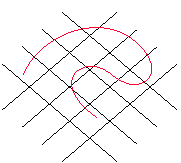
\includegraphics[width=2in]{main/Fig16-2-new}}
\caption{A curve of type (2,3) on a smooth quadric meets one ruling
twice and the other 3 times.}
\label{2,3 on quadric}
\end{figure}

\noindent{\bf Notation:} Throughout this section we consider the vector
bundle
$$
\sE = \sO_{\PP^1}(a_1) \oplus\sO_{\PP^1}(a_2)
$$
with  $0\leq a_1$, $1\leq a_2$ and  $a_{1}\leq a_{2}$. The
scroll $ S(a_1, a_2)$
lies in
$\PP^r` `$, where $r= a_1+a_2+1$. This scroll
is the image of $X = \PP(\sE)$ by a map that is an isomorphism
if $0<a_1$ and is the 
blowdown
\index{blowdown}%
of  $C_1$ if $a_1=0$.  We write $\pi:X
\to \PP^1$ for the projection, and
$C_{a_i}\subset X$ for the directrix of degree $a_i$. The degree of
$S(a_1,a_2)$ is $d \colonequals  a_1+a_2 = r-1$.

\subsubsection*{The case of a  smooth scroll}

Now assume in addition that $1\leq a_{1}$, so that $S(a_{1}, a_{2})$
is smooth.

\begin{theorem}\label{pic of scroll}

\begin{enumerate}

\item The 
Picard group
\index{Picard group}%
of $X = S(a_1,a_2)$ is $\Pic X \cong \ZZ^2``$, 
freely generated by  the class $F$ of a ruling and the class $H$
of a  hyperplane section.
\item The
intersection form on $\Pic(X)$ is given by
$$
\bordermatrix{\kern 10pt\cdot&F&H\cr
F&0&1\cr
H&1&d
}
\vspace*{3pt}
$$

\item The canonical class of the scroll is $K \colonequals  -2H +(d-2)F$,
so $K^2 = 8$.

\item The degree of a curve in the class $pH+qF$ is $pd+q$, while its
arithmetic genus is
$\tbinom{p}{2}@d+pq-p-q+1$.

\item The class of $C_{a_1}$
is $H-a_2F$, and the class of $C_{a_2}$
is $H-a_1F$.
\item If $C \subset \PP^{g-1}$ is a trigonal canonical curve and $X$
is the scroll swept out by the trisecants of $C$, then the class of $C$
is $3H+(4-g)F = H-K$.
\unif
\end{enumerate}
\end{theorem}

\begin{proof}
We have
$$
H^2 = \deg X = a_1+a_2 = d, \quad H.F = \deg F = 1, \quad F^2 = 0,
$$
where the last equality follows because any two fibers are linearly
equivalent and disjoint.
It follows 
that $H$ and $F$ are linearly independent.

We next show that $\Pic X$ is generated by $H$ and $F$. If $D$ is any
divisor,
then $D' = D - (F\cdot D)H$ meets $F$ in degree 0, and it now suffices
to show that $D'\sim aF$ for
some integer $a$.
Since $\sO_X(D')|_F = \sO_F$ for any fiber $F$, we see that
$\pi_*(\sO_X(D'))$ is a torsion-free sheaf on $\PP^1$ whose fiber at
each point is 1-dimensional,
so $\sL$ is a line bundle on $\PP^1` `$.  Possibly replacing $D'$ by
$-D'$, and using the fact that
$\pi_*(\sO_X(-D')) = (\pi_*(\sO_X(D'))^{-1}$, we may assume that $\sL$ is
globally generated, and it follows that  the natural map of line bundles
$\pi^*\sL = \pi^*\pi_* \sO_X(D') \to \sO_X(D') $ is a surjection, whence
$\sO_X(D') \cong \pi^*\sL$. Thus if $q = \deg \sL$ then
$D' \sim qF$. Note that we could also recover $q$ as $H\cdot D'$. This
completes the proof of parts
(1) and (2).

To compute the canonical class $K_X = pH+qF$ we use the adjunction
formula on the rational curves
$H$ and $F$. Thus $-2 = (F+K)\cdot F = p $ and
$$
-2 = (H+K)\cdot H = d + pd+q = d + (-2)d+q
$$
whence $q = d-2$ as required for part (3).

Part (4) is a direct computation from the adjunction formula.

For part (5) we observe that a hyperplane containing $C_{a_1}$ meets $X$
in $C_{a_1}$ plus
$a_2$ rulings; thus $C_{a_1}\sim H-a_2F$. Similar reasoning holds for
$C_{a_{2}}$.

If  $C \subset S(a_{1}, a_{2}) \subset \PP^{g-1}$ is a	trigonal canonical
curve of genus $g$, then the degree
$d$ of the scroll must be $g-2$. Moreover $C.F=3$ and $C.(C+K) =
2g-2$. These equations have the unique solution
$C \sim H-K = 3H + (4-g)F$.
\end{proof}

Now we can say exactly which classes on the scroll contain curves:

\begin{theorem}\label{where are the curves?} Again, suppose that
$0<a_{1}$.
There are reduced  curves in the class $D = pH+qF$ if and only~if one
of the following holds:

\begin{enumerate}
\item $D\sim qF$; that is, $p=0, q>0$.
\item $D\sim C_{a_{1}}$; that is, $p=1, q=-a_{2}$.
\item $p\geq 0$ and $D\cdot C_{a_{1}}> 0$; that is, $q \geq -pa_1$.
\end{enumerate}
In case (3) the linear series $|D|$ is 
basepoint free. 
\index{basepoint free}%
When, in addition,
$a_2>a_1$ or $q>-pa_1$ the class $|D|$ contains irreducible smooth curves.
\unif
\end{theorem}

Note that in case (1) we have $D^{2} = 0$, because any two fibers of $\pi$
are disjoint; in case (2) we have $D^{2}= a_{1}-a_{2}\leq 0$ and in case
(3) we have $D^{2}\geq 0$, and $D^2=0$ only~if
$d=2, q = -pa_1$. In particular, no irreducible curve
on $X$ other than $C_{a_1}$ can have negative self-intersection.

\begin{proof}
The existence of smooth curves of types (1) and (2) is obvious; the following
result will show that
the ones of type (3) move in a basepoint free linear series. By 
Bertini's theorem
\index{Bertini's theorem}%
(Theorem \ref{Bertini}), such a series must contain smooth curves unless the
associated map factors through a curve, in which case $D^2 = dp^2-2pq =
p(pa_1+pa_2 -2 q) = 0$, which implies that $a_2=a_1$ and $q= -pa_1$.

Theorem~\ref{global sections}, below, thus completes the proof.
\end{proof}

\begin{theorem}\label{global sections} Again, suppose that $0<a_{1}$.
Suppose that $D$ is a divisor on the scroll $X$ as above. If $D \sim
pH+qF$ is effective,  then $p\geq 0$ and
$$
H^{0}(\sO_{X}(D)) = H^{0}(\sO_{\PP^{1}}(q) \otimes \Sym^{p} \sE)
=
\tsty\bigoplus\limits_{0\leq i\leq p}H^{0}\bigl(\sO_{\PP^{1}}(q + (p-i)a_{1}+i
a_{2})\bigr).
$$
The linear series $|D|$ is basepoint free if and only~if every summand
\index{basepoint free}%
in the last expression is nonzero.
Thus, numerically,
$$
h^{0}(\sO_{X}(D)) =
\sum_{i @\mid@ q+(p-i)a_{1}+i a_{2} \geq 0}1+(q + (p-i)a_{1}+i a_{2}),
$$
and
$|D|$ is basepoint free if and only~if $p\geq 0$ and $q\geq -pa_{1}$.
\unif
\end{theorem}

\begin{proof} First, If $q<-pa_{1}$, then
$$
D\cdot C_{a_{1}} = (pH+qF) \cdot (H-a_{2}F) = p(a_{1}+a_{2}) -pa_{1}+q =
pa_{1}+q < 0,
$$
so any effective divisor in the class of $D$ must have a component in
common with $C_{a_{1}}$.

Let $\pi:X\to \PP^{1}$ be the structure map of the projective bundle $X
= \PP_{\PP^{1}}(\sE)$.
We have $H^{0}(\sO_{X}(pH+qF)) = H^{0}(\pi_{*}(\sO_{X}(pH+qF)))$. Also,
we may write $\sO_{X}(pH+qF)$ as $\sO_{X}(p) \otimes
\pi^{*}\sO_{\PP^{1}}(q)$, and since
$\sO_{\PP^{1}}(q)$ is a line bundle we see that
$$
\pi_{*}\bigl(\sO_{X}(p) \otimes \pi^{*}\sO_{\PP^{1}}(q)\bigr)
= \pi_{*}\bigl(\sO_{X}(p)\bigr)\otimes \sO_{\PP^{1}}(q).
$$

The projective bundle $\PP(\sE)$ is
by definition Proj of the symmetric algebra $\PP(\sE)\colonequals
\Proj(\Sym \sE)$. Over any open
subset $U$ of the base $\PP^1$ over which $\sE$ is free, this is
$\pi^{-1}(U) = U\times \PP^1` `$,
and it follows that $\pi_*(\sO_{\PP(\sE)}(p)) = \Sym^p\sE$.
Thus
\begin{align*}
\pi_{*}(\sO_{X}(pH+qF)) &=
\pi_{*}\bigl(\sO_{X}(p) \otimes \pi^{*}\sO_{\PP^{1}}(q)\bigr) \\
&= \pi_{*}\bigl(\sO_{X}(p)\bigr)\otimes \sO_{\PP^{1}}(q)
=  \Sym^{p} \sE\otimes \sO_{\PP^{1}}(q)\\
&=  \bigl(\tsty\bigoplus\limits_{0\leq i\leq p}\! \sO_{\PP^{1}}((p-i)a_{1}+i
a_{2})\bigr) \otimes \sO_{\PP^{1}}(q),
\end{align*}
and the first formula follows.

The term
$H^{0}(\sO_{\PP^{1}}(q + (p-i)a_{1}+i a_{2}))$ is nonzero for all $i$
if and only~if
$H^{0}(\sO_{\PP^{1}}(q + pa_{1}))$ is nonzero, which holds if and only~if
$q\geq -pa_{1}$.
If $\sigma = \sum \sigma_i$ is a section of $\sO_X(D)$ written according
to the decomposition
above, then the restriction of $\sigma$ to  the rational normal curve
$C_{a_1} = \PP(\sO_{\PP^1}(a_1))$ is the component $\sigma_0$, and
similarly for $C_{a_2}$ and $\sigma_p$. Thus when  all the summands
are nonzero
there are sections  vanishing on $C_{a_{1}}$ but not $C_{a_{2}}$, and
vice versa, so the system is basepoint free.
\index{basepoint free}%
\end{proof}

\subsubsection*{The case of a 
singular scroll
$S(0,a_{2})$}

\index{singular scroll}%
We now assume that $a_{1} = 0$. We will use a general fact about
projective bundles:

\begin{proposition}\label{singular scrolls}
If $X$ is a scheme, $\sE$ a locally free sheaf on $X$, $\sL$ an invertible
sheaf on $X$
and $\pi: \PP(\sE)\to X$ the natural projection.
Under the isomorphism
$$
\PP(\sL \otimes \sE)\cong \PP(\sE)
$$
the invertible sheaf $\sO_{\PP(\sE\otimes \sL)}(1)$ corresponds to the
invertible sheaf
$$\sO_{\PP(\sE)}(1)\otimes \pi^{*}\sL.$$

Moreover, the singular scroll $S(0,a_{2})$, which is the cone over a
rational normal curve of degree $a_{2}$, is the image of
$S(1, a_{2}+1)$ under the map corresponding to the complete linear series
$$
\bigl|\sO_{S(1, a_{2}+1)}(1) \otimes \pi^{*}(\sO_{\PP^{1}}(-1))\bigr|,
$$
which 
blows down
\index{blowdown}%
the line $C_{1}$.
\unif
\end{proposition}

Note that $S(1,a_2+1)$ is isomorphic to the surface $\tilde S(0, a_2)$
of Section~\ref{daily name}.

\begin{proof}
The isomorphism $\PP(\sE) \to \PP(\sE\otimes \sL)$ corresponds to the
surjection
$$\pi^*(\sE \otimes\sL) \cong \pi^*(\sE) \otimes \pi^*(\sL) \to
\sO_{\PP(\sE)}(1) \otimes \pi^*(\sL),$$
and the inverse map is formed similarly.

When $\sE = \sO_{\PP^1}(a_1)\oplus \sO_{\PP^1}(a_2+1)$ and $a_1 = 1$ the
invertible sheaf
$$
\sO_{S(a_1, a_{2}+1)}(1) \otimes \pi^{*}(\sO_{\PP^{1}}(-1))
$$
corresponds to the divisor class $H-F$, which meets $C_{a_1}$	in degree
0, so the image
of $C_{a_1}$ under the corresponding linear series is a point. However
the description of  $H^0(\sE)$ in
Theorem~\ref{global sections} shows that the restriction to $F$
is still the complete linear series $|\sO_{\PP^1}(1)|$, and the
restriction to $C_{{a_2}+1}\cong \PP^1$
is $|\sO_{\PP^1}(a_2+1)|$. Thus the displayed linear series in the
proposition is basepoint free and
does define a map as claimed.
\end{proof}

\begin{theorem}\label{curves on a singular scroll}
Suppose that $C$ is a smooth curve lying on the scroll $S(0,d)$, with
$1\leq d$. Let $H,F$ be the 
(Weil) divisor classes 
\index{Weil divisor}%
of the hyperplane
section and ruling, respectively.
\begin{enumerate}
\item $C\sim mH$ or $C\sim mH+F$ for some $m\geq 0$.
\item If $C\sim mH$ then $\deg C = md$ and the genus of $C$ is $g =
\tbinom{m}{2}d-m+1$.
\item If $C\sim mH+F$ then $\deg C = md+1$ and the genus of $C$ is $g =
\tbinom{m}{2}d$.
\end{enumerate}
In particular, $\deg C$ is congruent to 0 or 1 modulo $d$.
\unif
\end{theorem}

\begin{proof}
\noindent $d=1$: In this case, $S(0,1)\cong \PP^{2}$, with a distinguished
point $\phi_{1}(\PP^{1})$ and $mH+F = (m+1)H$.
The formulas for degree and genus are familiar from the theory of curves
in the plane.

We now assume $2\leq d$, so $S(0,d)$ is a cone over the rational normal
curve of degree $d$. Let $\pi: S(1,d+1) = \tilde S(0,d) \to S(0,d)$
be the blowup of the vertex of the cone, and let $E,L$ be the exceptional
divisor and ruling on $S(1, d+1)$,
so that $E = C_{1}$ and $E^{2} = -d$. The proper transform of the
hyperplane class $H$ on $S(0,d)$ has intersection number 1 with $L$
and $0$ with $E$,
and is thus of class $E+dL$. Let $\tilde C \cong C$ be the proper
transform of $C$ on $S(1,d)$.
Since $C$ is smooth, $\tilde C$ meets $E$ at most once, whence the
first assertion.

The degree assertions of items 2,3 are immediate, and the genus assertions
follow by direct computation from the
adjunction formula on $S(1,d+1)$.
\end{proof}

In these terms we can also see which classes on a singular scroll
correspond to 
hyperelliptic
\index{hyperelliptic curve}%
 or canonical 
trigonal
\index{trigonal}%
 curves in the way
described by Corollary~\ref{hyperelliptic and trigonal}:

\begin{corollary}\label{which class}
\begin{enumerate}
\item For a smooth canonical curve $C\subset \PP^{g-1}$ to lie on a
singular scroll it is necessary that $g\leq 4$.
If $g=4$ then $C$ is a complete intersection of the cone over a conic
with a cubic surface not passing through
the vertex of the cone; thus $C$ is trigonal, as is also the case
for $g=3$.

\item If  $C$ is a smooth hyperelliptic curve of genus $g\geq 2$, and
the union of the secant lines to $C$ corresponding to the
hyperelliptic involution sweep out 
a singular scroll $S(0,d)$ then
$C\sim 2H$ or $2H+F$ on $\tilde S(0,d) = S(1,d+1)$ in which cases
the degree of $C$ is $2d$ or $2d+1$ and the genus of $C$ is $d-1$ or $d$
respectively. Conversely,
any  curve in these classes is hyperelliptic and the lines on the singular
scroll	$S(0,d)\subset \PP^{d}$
meet the image of $C$ in the pairs of points that are conjugate under
the hyperelliptic involution.
\unif
\end{enumerate}
\end{corollary}

\begin{proof} (1)\, If $C\subset \PP^{g-1}$ is a smooth nonhyperelliptic
canonical curve lying on a singular 2-dimensional scroll in $\PP^{g-1}$
then the scroll is $S(0, g-2)$. By Theorem~\ref{curves on a singular
scroll}, $\deg C = 2g-2$ must be congruent
to 0 or 1 modulo $g-2$, and this is the case only for $g=3,4$, the cases
of a plane quartic or the complete intersection
of a quadric cone with a cubic surface not passing through the vertex
of the cone.

\noindent
(2)\, By hypothesis the 
strict transform
\index{strict transform}%
$\tilde C\subset  \tilde S = S(1, d+1)$
has class $2H+\epsilon F$,  and by Theorem~\ref{curves on a singular
scroll}, $\epsilon$ is 0 or 1.
The formulas for degree and genus follow are given in that theorem.
\end{proof}

\section{Exercises}

\begin{exercise}\label{special projections}
Suppose $1\leq a_1 < a_2$. Show that the projection of $S(a_1,a_2)$
from any point on $C_{a_1}$ is
$S(a_1-1, a_2)$, and that the projection from any point on $C_{a_2}$
is $S(a_1, a_2-1)$. (If $a_1 = a_2$, projection of $S(a_1,a_2)$ from
any point is $S(a_1-1, a_2)$.)

This gives another proof that the blowup of the cone $S(0,a_2)$ over
the rational normal curve of degree $a_2$ is $S(1,a_2+1)$.
\end{exercise}

\begin{exercise}
Show that a matrix $M$ of linear forms is 1-generic if and only~if,
even after arbitrary row and column transformations, its entries are
all nonzero.
\end{exercise}

\begin{exercise}
Let $M$ be a 1-generic $p\times q$ matrix of linear forms, with $p\leq
q$. Show that the codimension of
$I_p(M)$ is $q-p+1$. 
\tohint{17.3}
\end{exercise}

\begin{exercise}
Show that if $X\subset \PP^r$ is a projective variety whose homogeneous
ideal $I$ contains $m$ independent quadrics, then the ideal of the
general hyperplane section of $X$ in $\PP^{n-1}$
contains at least $m$ independent quadrics. Use this to prove that if $X$
has codimension $c$ then $m\leq \tbinom{c+1}{2}$, and that equality holds
if and only~if
$X$ is a variety of minimal degree (that is, $\deg X = c+1$.)
\end{exercise}

\begin{exercise}\label{many quadrics}
If $X \subset \PP^r$ is an irreducible, nondegenerate projective variety
of codimension $c$ whose homogeneous ideal
contains $\tbinom{c}{2}$ independent quadratic forms, then $X$ is a
variety of degree $c$.
\tohint{17.5}
\end{exercise}

\begin{exercise}\label{Castelnuovo Veronese}
Show that every reduced, irreducible curve on the Veronese surface is
\index{Veronese!surface}%
\index{Castelnuovo curve}%
a Castelnuovo curve.
\end{exercise}

\begin{exercise}\label{cohomology of invertible sheaves on a scroll}
\begin{enumerate}
\item
Use the Leray spectral sequence
\index{Leray spectral sequence}%
 to compute the cohomology
$H^{i}(\sO_{X}(D))$ on a scroll $X\subset \PP^r`$.
\item
Using this, show that $X$ is arithmetically Cohen--Macaulay.
\tohin{17.7}
\index{ACM}%
\end{enumerate}\label{tnih17.7}
\end{exercise}

\begin{exercise}
Show that if $X\subset\PP^r$ is an arithmetically Cohen--Macaulay surface
and $D\subset X$ is a curve, then $D$ is arithmetically Cohen--Macaulay
if and only~if
$H^1_*(\sI_{D/X}) = 0$. Use this and Exercise~\ref{cohomology of
invertible sheaves on a scroll} to determine the
possible divisor classes of arithmetically Cohen--Macaulay curves on a
2-dimensional scroll.
\end{exercise}

\begin{exercise}\label{Castelnuovo scrolls}
By Theorem~\ref{Castelnuovo's bound}  Castelnuovo curves are
arithmetically Cohen--Macaulay.
Show that all the arithmetically Cohen--Macaulay curves on a 2-dimensional
scroll are
Castelnuovo curves.
\index{Castelnuovo curve}%
\tohint{17.9}
\end{exercise}

\begin{exercise}
State and prove an analogue of Proposition~\ref{which scroll} for curves
on scrolls of dimension $>2$.
\tohint{17.10}
\end{exercise}

\begin{exercise}\label{general projections}
Improve the result of Exercise~\ref{special projections} by showing that,
if $0\leq a_1\leq a_2$, then
the projection of $S(a_1,a_2)$ from any point not on $C_{a_1}$ (or not
the vertex, in case $a_1=0$) is
$S(a_1, a_2-1)$.
\end{exercise}

\begin{exercise}\label{curves on cones}
\begin{enumerate}
\item If $C \subset S(0, a_2) \subset \PP^{a_2+1}$ is a smooth curve
with class $m$ times the hyperplane section (i.e., corresponding to
a curve on $S(1,a_2+\nobreak 1)$ with class $mH - mF$), show that
$$
\deg C = ma_2 \quad \text{and} \quad g(C) = \tbinom{m}{2}@a_2 - m + 1.
$$
\item If $C \subset S(0, a_2) \subset \PP^{a_2+1}$ is a smooth curve
with class $m$ times the hyperplane section plus a ruling (i.e.,
corresponding to a curve on $S(1,a_2+1)$ with class $mH - (m-1)F$),
show that
$$
\deg C = ma_2 + 1 \quad \text{and} \quad g(C) = \tbinom{m}{2}@a_2.
$$
\end{enumerate}
\end{exercise}

\begin{exercise}~\label{2r+3 is sharp}
Show that 3 general quadrics meet in 8 points in $\PP^3$ that do not
lie on a twisted cubic, and deduce that the bound $d \geq 2r+3$ in
Theorem~\ref{Castelnuovo2r+3}
is sharp.
\end{exercise}

\begin{exercise}[trigonal curves of genus 5]
\label{extrigonal genus 5}
In
our study of canonical curves of genus 5 (second case,
page~\pageref{trigonal genus 5})
we analyzed 
trigonal curves $C\subset \PP^4$ of genus 5,
\index{trigonal!curve of genus 5}%
showing that
there are three independent quadrics in $I_C$ that are either a complete
intersection (and generate $I_C$ or
meet in a nondegenerate surface). From Corollary~\ref{hyperelliptic and
trigonal} we know that in the second case
the surface is a scroll. Complete the analysis by deciding between the
two types of scrolls in $\PP^4$: $S(1,2)$ and $S(0,3)$.
What is the divisor class of the curve on the scroll?
\tohint{17.14}
\end{exercise}

\begin{exercise}\label{Maroni Bound}
If $C$ is a smooth 
\index{trigonal}%
trigonal curve, 
canonically embedded in $\PP^{g-1}$,
then
$C$ lies on a 2-dimensional scroll $S(a_1, a_2)$, as in
Theorem~\ref{pic of scroll}. Show that
$$
a_2-a_1\leq \frac{g+2}{3}.
$$
(In this situation the difference $|a_2-a_1|$ is called the 
\index{Maroni invariant}%
\emph{Maroni invariant}.)
\tohint{17.15}
\index{scroll|)}%
\end{exercise}


